\documentclass[a4paper,12pt]{article}

\usepackage[utf8]{inputenc}
\usepackage[T1]{fontenc}
\usepackage{graphicx}
\usepackage{geometry}
\usepackage{subcaption}
\usepackage{setspace}
\usepackage{minted}
\usepackage{authblk}
\usepackage{caption}
\captionsetup[listing]{labelformat=empty}
\usepackage{amsmath}
\usepackage{amssymb}
\usepackage{regexpatch}
\usepackage{dsfont} 
\usepackage{mathrsfs}
\usepackage{array}
\usepackage{hyperref}
\usepackage{tikz}
\usetikzlibrary{trees}
\usetikzlibrary{positioning}
\usepackage{xcolor}
\usepackage{pgfkeys}
\usepackage{booktabs}
\usepackage{listings}
\usepackage[linesnumbered,ruled,vlined]{algorithm2e}
\usepackage[noend]{algpseudocode}
\usepackage{fancyhdr}
\setlength{\parindent}{0pt}
\geometry{a4paper, margin=2.5cm}

\sloppy
\begin{document}

\begin{titlepage}

    \vspace*{4cm}

    \centering
    
    
\includegraphics[width=0.6\textwidth]{Images/logo.png} \\[1.5cm]
    
    \rule{\linewidth}{1pt} \\[1cm]

    {\Huge \bfseries HAX907X - Apprentissage statistique}\\[0.5cm]
    {\Huge TP : Support Vector Machines (SVM)}\\[1cm]
    
    \rule{\linewidth}{1pt} \\[2cm]

    {\Large \textbf{Marine GERMAIN}}\\
    {\Large \textbf{Coralie ROMANI DE VINCI}}\\[1cm]
    

\end{titlepage}


\renewcommand{\contentsname}{Table des matières}
\tableofcontents


\newpage

\section{Base de données Iris}

Dans cette section nous étudierons la base de données Iris sur laquelle nous ferons une étude de classification sur les classes $1$ et $2$.
Nous utiliserons d'abord le noyau linéaire puis le noyau polynomial et nous les comparerons.
Nous avons séparé le dataset en deux parties : un ensemble d'entraînement (75\% des données) et un ensemble de test(25\% des données). 

\subsection{Classification avec noyau linéaire}

La classification des deux premières variables avec un noyau linéaire à pour objectif de trouver une hyperplan qui sépare au mieux les deux classes en maximisant la marge entre les points les plus proches de chaque classe. 
Les scores obtenues pour cette méthode sont les suivants :

\begin{figure}[h!]
    \centering
    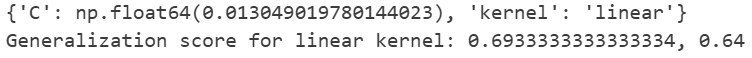
\includegraphics[width=0.8\textwidth]{Images/linear_score.png}
    \caption{}
    \label{fig:linear}
\end{figure}

Pour les données d'entraînement, le modèle à classfié correctement 77,3\% des données, contre 64\% pour les données de test. 


\subsection{Classification avec noyau polynomial}

La classification des deux premières variables avec un noyau polynomial à pour objectif de trouver une frontière de décision non linéaire capable de séparer au mieux les deux classes. 
Les scores obtenues pour cette méthode sont les suivants :

\begin{figure}[h!]
    \centering
    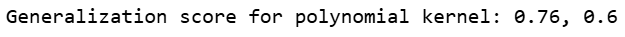
\includegraphics[width=0.8\textwidth]{Images/poly_score.png}
    \caption{}
    \label{fig:poly}
\end{figure}

Pour les données d'entraînement, le modèle à classfié correctement 76\% des données, contre 60\% pour les données de test. \\

\textbf{Comparaison des deux méthodes :}\\[0.5cm]
- Nous disposons d'abord, des scores respectifs obtenues en figure \ref{fig:linear} et figure \ref{fig:poly}.
On remarque que le score pour le noyau linéaire est plus élevé que celui du noyau polynomial, autant pour les données d'entraînements que pour les données de test.\\

- Ensuite, nous avons tracé graphiquement ces résultats à l'aide des frontières : 
\begin{figure}[h!]
    \centering
    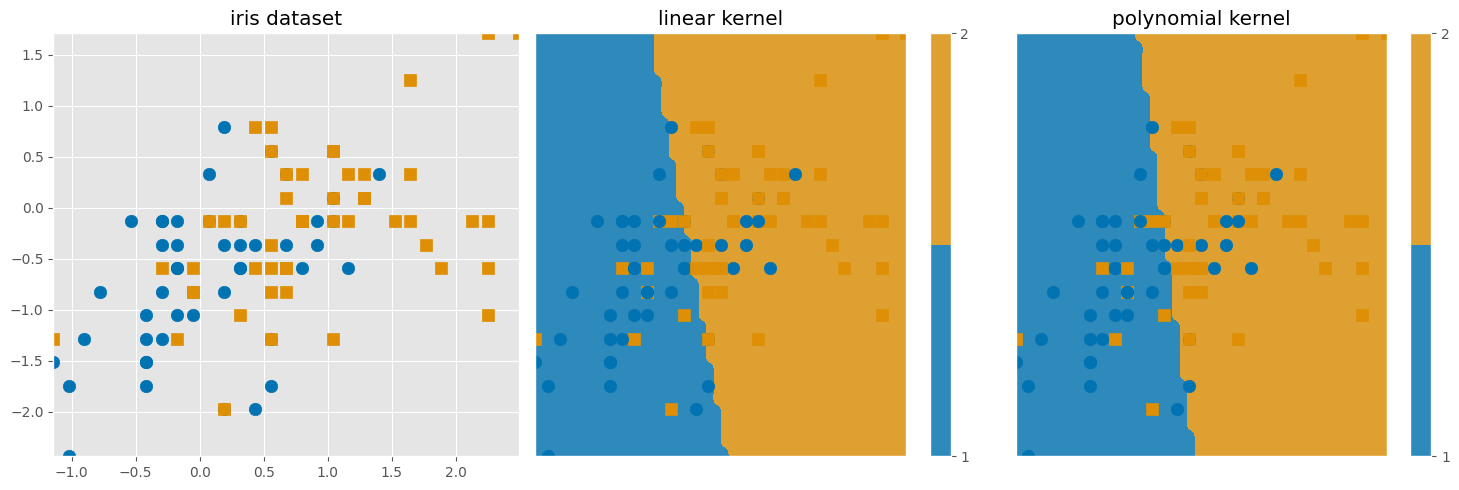
\includegraphics[width=0.8\textwidth]{Images/linear_vs_poly.png}
    \caption{}
\end{figure}

\section{SVM GUI}

\section{Classification des visages}

\subsection{Influence du paramètre de régularisation}

\subsection{Variable de nuisances}

\subsection{Réduction de dimension}

\end{document}